\documentclass[a4paper,parskip]{scrartcl}

\usepackage{lmodern}
\renewcommand*\familydefault{\sfdefault}
\usepackage[T1]{fontenc}

\usepackage[ngerman]{babel} %german english spell checking
\usepackage[utf8]{inputenc} %allows ä,ö,ü and others
\usepackage{multicol} %allows multiple columns
\usepackage{enumitem} %allows to change enumerate style
\usepackage[colorlinks=true,pdfborder={0 0 0},urlcolor=cyan,linkcolor=black]{hyperref} %allows links
\usepackage{verbatim} %allows code
\usepackage{graphicx} %allows images
\usepackage{amssymb} %allows symbols for number sets

\setlist{nosep} %smaller lists, less space between lines

\title{Anforderungs- Dokumentation}
\author{Lorenz Rasch \& Dominik Meister}

\begin{document}
\maketitle
\tableofcontents
\pagebreak

\section{Ziel des Dokumentes}
FIXME

\section{Vision}
Jeder kennt diese Situation, man sitzt in einem Meeting und möchte kurz ein Brainstorming machen. Oder man
möchte für die nächste Arbeit zu einem Thema eine Übersicht zu den Informationen erstellen.
Eine der einfachsten Methoden so eine Übersicht darzustellen ist das Mindmap. Das Mindmap auch Gedankenlandkarte genannt ist eine Technik welche von Tony Buzan geprägt und entwickelt wurde.
Das Mindmap basiert auf dem Prinzip der Assoziation. Dies kommt nicht von ungefähr, unser Gehirn arbeitet ebenfalls mit Assoziationen, es versucht ständig neue Informationen mit gewissen Kategorien und anderen Informationen zu verknüpfen. Das Mindmap basiert auf derselben Technik, deshalb fällt es uns auch sehr einfach ein Mindmap zu erstellen.
Dieses zu erstellen ist jedoch mit den meisten Programmen eher mühsam, deshalb greift man auf den Stift und Papier zurück. Um hier Abhilfe zu schaffen kommt unser Projekt ins Spiel.
\newpage
\section{Ziel des Projektes}
Ziel unseres Projektes ist, die Erstellung einer einfachen und performanden Mindmap Software. Sie soll
den Menschen helfen Ihre Ideen einfach in Form eines Mindmapes darzustellen und abzuspeichern.\\
\begin{itemize}
\item Wirtschaftlich
	\begin{itemize}
	\item Mithilfe des Programmes kann viel Zeit beim erstellen des Mindmaps gespart werden.
	\item Durch das digitale Abspeichern besteht auch die Gefahr des Verlierens weniger als, bei einem Mindmap auf Papier.
	\end{itemize}
\item System
	\begin{itemize}
	\item Das System unterstützt den Benutzer beim Erstellen möglichst übersichtlichen Mindmaps.
	\item Das System kann Mindmaps zu Bildern exportieren und diese auch ausdrucken, damit sie weiterverwendet werden können.
	\end{itemize}
\item Personell
	\begin{itemize}
	\item Das Programm soll selbsterklärend sein und keine Anleitung benötigen.
	\item Das Programm soll ohne Experten installiert werden können.
	\end{itemize}
\item Qualität
	\begin{itemize}
	\item Das Programm soll weniger komplex aufgebaut sein, als die meisten anderen Mindmap Applikationen
	\item Das Programm soll durch verschiedene Verbindungstypen und Farben Übersichtlichere Mindmaps generien können.
	\end{itemize}

\end{itemize}
\newpage


\section{System Kontext}
Der Systemkontext ist eine Beschreibung des Systems, seiner Teile und äusserlichen Einwirkungen auf das System.
Der Benutzer kann mit unserer Software ein Mindmap erstellen. Dies geschieht über eine grafische Benutzeroberfläche. Mit Hilfe eines Algorithmus können die Themen und Verbindungen des Mindmap optimal verteilt werden. Die Benutzeroberfläche und der Algorithmus sind Teil der Software\\
Die Software greift auf das Dateisystem des Computers zu um ein Mindmap zu speichern oder zu laden.
Der Druckservice des Computers erlaubt das Drucken des Mindmaps. Diese beiden Teile liegen ausserhalb unserer Software.

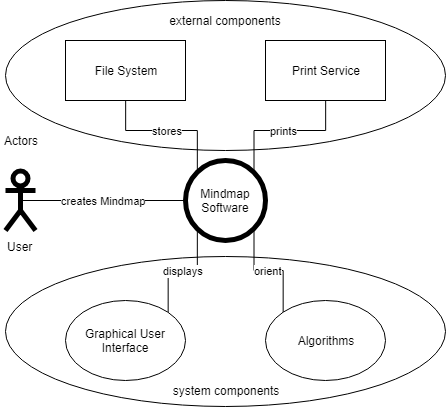
\includegraphics[width=0.5\linewidth]{Systemkontext.png}

\newpage

\section{Anforderungen}

\subsection{Nichtfunktionale Anforderungen}

\begin{table}[h]

\begin{tabular}{|l|l|l|l|l|l|l|}

\hline
Nr  & Datum   & Beschreibung                 & P & K & V & R \\ \hline
1.1 & 14.3.19 & Benutzerfreundlich           &   &   &   &   \\ \hline
1.2 & 14.3.19 & Schnell / Effizient          &   &   &   &   \\ \hline
1.3 & 14.3.19 & Optisch ansprechendes Design &   &   &   &   \\ \hline
1.4 & 14.3.19 & Output wie Input             &   &   &   &   \\ \hline
1.5 & 14.3.19 & Einfache Installation        &   &   &   &   \\ \hline
\end{tabular}
\end{table}

\begin{enumerate}
\item [1.1] Als Benutzer möchte ich, dass das Programm selbsterklärend und einfach zu bedienen ist.
\item [1.2] Als Benutzer möchte ich ein Programm welches schnell startet und sich nicht langsam anfühlt.
\item [1.3] Als Benutzer möchte ich ein optisch Ansprechendes Design. Als Benutzer finde ich ein Programm
besser wenn sein Design State of the Art ist.
\item [1.4] Als Benutzer möchte ich, dass das Mindmap auf dem Papier gleich aussieht wie es im Programm ausgesehen hat.
\item [1.5] Als Benutzer möchte ich nicht einen Experten konsultieren müssen um ein so triviales Programm zu installieren. 
\end{enumerate}

\subsection{Funktionale Anforderungen}
\begin{table}[h]

\begin{tabular}{|l|l|l|l|l|l|l|}

\hline
Nr  & Datum   & Beschreibung                        & P & K & V & R \\ \hline
2.1 & 14.3.19 & Neues Mindmap erstellen             &   &   &   &   \\ \hline
2.2 & 14.3.19 & Knoten hinzufügen                   &   &   &   &   \\ \hline
2.3 & 14.3.19 & Knoten miteinander verbinden        &   &   &   &   \\ \hline
2.4 & 14.3.19 & Mindmaps speichern/laden            &   &   &   &   \\ \hline
2.5 & 14.3.19 & Beschreibung eines Knoten anpassen  &   &   &   &   \\ \hline
2.6 & 14.3.19 & Farbe eines Knoten ändern           &   &   &   &   \\ \hline
2.7 & 14.3.19 & Verschiedene Verbindungstypen       &   &   &   &   \\ \hline
2.8 & 14.3.19 & Drucken eines Mindmaps              &   &   &   &   \\ \hline
2.9 & 14.3.19 & Exportieren eines Mindmaps          &   &   &   &   \\ \hline
2.10 & 14.3.19 & Optimale Verteilung der Knoten      &   &   &   &   \\ \hline

\end{tabular}

\end{table}

\begin{enumerate}
\item [2.1] Als Benutzer möchte ich mit dem Programm neue Mindmaps erstellen können.
\item [2.2] Als Benutzer möchte ich neue Knoten hinzufügen könnnen, welcher eine Beschreibung besitzt und wenn gewünscht auch eine spezielle Farbe haben kann. 
\item [2.3] Als Benutzer möchte ich die verschiedenen Informationen, also Knoten miteinander vernetzen und so grupieren können. 
\item [2.4] Als Benutzer möchte ich meine Arbeit speichern können und gespeicherte Projekte auch wieder laden können
\item [2.5] Als Benutzer möchte ich die Beschreibung eines Knoten auch nach seiner Erstellung bearbeiten können.
\item [2.6] Als Benutzer möchte ich die Farbe eines Knotens nach seiner Erstellung bearbeiten können.
\item [2.7] Als Benutzer möchte ich verschiedene Verbindungstypen definieren können, ich möchte Verbindungen zwischen verschiedenen Themen speziell hervorheben können. 
\item [2.8] Als Benutzer möchte ich mein Mindmap drucken können.
\item [2.9] Als Benutzer möchte ich mein Mindmap exportieren können, um es zum Beispiel als Bilddatei in einem Worddokument einfügen zu können.
\item [2.10] Als Benutzer möchte ich ein Mindmap mit möglichst wenigen überschneidenden Verbindungen, das Programm sollte eine Möglichkeit bieten dieses Problem zu lösen.
\end{enumerate}

\section{Glossar}

\end{document}
